\chapter{Surrogate Assisted Optimization}
\label{chapter:3}

\begin{tcolorbox}
\textit{The works presented in this chapter have been published in the following articles:}
\begin{enumerate}
\small
\item \textbf{Islam,~M.~M.}, {Singh,~H.~K.},  {Ray,~T.}, and {Sinha,~A.} ``An Enhanced memetic algorithm for single-objective bilevel optimization problems,'' {\em Evolutionary Computation}, MIT press, 2016~\textbf{(Impact factor: 3.6)}.
\item \textbf{Islam,~M.~M.}, {Singh,~H.~K.}, and {Ray,~T.}, ``A Memetic Algorithm for Solving Bilevel Optimization Problems with Multiple Followers,,'' in {\em Proceedings of IEEE Congress on Evolutionary Computation (CEC)}, Vancouver, Canada, pp. 1901--1908, 2016.
\item  \textbf{Islam,~M.~M.}, {Singh, H.K.} and {Ray, T.}``A Memetic Algorithm for the Solution of Single Objective Bilevel Optimization Problems,,'' in {\em Proceedings of IEEE Congress on Evolutionary Computation (CEC)}, Sendai, Japan, pp. 1643-1650, 2015.

\end{enumerate}

\end{tcolorbox}


\section{Introduction}
\label{sec:intro}






\section{Background}
\label{sec:back}

\section{SAMO}

\section{Introduction}

Evolutionary algorithms~(EAs) have long been a preferred choice for solving multi-objective optimization problems as they can deliver a set of non-dominated solutions in a single run closely representing the Pareto optimal front~(POF).  Furthermore, since EAs do not require assumptions on continuity and differentiability of the underlying objective and constraint functions, they can be applied to a wide range of problems. However, being population based methods, EAs require evaluation of numerous solutions before converging to the POF. This becomes computationally prohibitive for problems where evaluation of each candidate design involves computationally expensive analysis, such as computational fluid dynamics~(CFD), finite element analysis~(FEA), computational electromagnetics~(CEM), etc. Thus there is a growing interest in the use of approximation models~(referred to as meta-models, surrogate models or simply surrogates) to guide the search in order to reduce the number of true function evaluations.

A review of the methods used for fitness approximation appears in \cite{wang_review_2007} and a survey on the use of fitness approximation in the context of evolutionary computation has been reported in \cite{jin2005csf}. A number of different surrogate models have been established and chosen for different studies in literature. These include neural network based models like multi-layer perceptrons, radial basis function networks, quadratic response surfaces, Kriging and CoKriging models. A vast majority of surrogate assisted optimization methods use a single type of global surrogate model to represent each objective and constraint function. The surrogate model is either created once and used subsequently throughout the course of search, or created/updated periodically. Algorithms which only build the surrogate once~\cite{wilson2001epf,goel_ensemble_2007} rely significantly on the quality of initially sampled solutions to generate the model. Periodic re-training of the surrogate model is usually necessary as the search intensifies in localized areas. In order to capture local behavior, hierarchical surrogate models have been introduced in \cite{zhou_combining_2007}. Construction of hierarchical surrogate models by space reduction using fuzzy clustering has also been reported in \cite{wang_fuzzy_2004}.

To improve the prediction accuracy with limited samples, multiple surrogates can be used in place of a single surrogate model. Common use of multiple surrogates is in the form of surrogate \textit{ensembles}, where a collection of surrogate models with varying parameters are trained simultaneously by techniques such as bagging~\cite{breiman_bagging_1996} and boosting~\cite{abney_boosting_1999}. In \cite{acar2010ensemble}, an ensemble was constructed using a weighted aggregation with the weight factors identified using point-wise cross validation error. A survey of neural network ensembles appear in~\cite{zhao_survey_2005}. It is important to highlight that the above reports focus on construction of surrogate models/ensembles only. In the context of optimization, subsequent management of the surrogate models during the course of the search while avoiding ill-validation is of critical importance as highlighted in\cite{jin2005csf}. In the context of surrogate assisted optimization, aggregation principles have also been suggested in~\cite{goel_ensemble_2007,zerpa_optimization_2005, hamza2012co}, where a weighted average model resulting from various surrogate types (polynomial response surface model, Kriging, and radial basis function) was used. 

Weighted aggregation has also been used in conjunction with multiple surrogates for single objective optimization~\cite{glaz2009rotor} and multi-objective optimization~\cite{mack2005bluff}. There are also reports of surrogates constructed using a global~(trend) model and a local model~\cite{goel2006perf, zhou_memetic_2007} for single objective optimization. In \cite{zhou_combining_2007}, a radial basis function was used as a local surrogate while a Kriging model was used as a global surrogate. Once again, the above study was restricted to single objective unconstrained optimization problems only.

In the context of multi-objective optimization, a multi-layer perceptron was periodically re-trained and used alternatively with actual computations to solve a B-spline curve fitting problem~\cite{nain_computationally_2002}. A similar approach of alternating between actual analysis and surrogate models has also been reported in~\cite{ray2006sae}. Pareto Efficient Global Optimization~(ParEGO) algorithm~\cite{knowles2006pha} is yet another class of methods, where a Kriging based surrogate is constructed and the sampling points are identified via an optimization process. However, the method requires knowledge about the limits of the objective function space. In \cite{chafekar2005mgo}, use of multiple Genetic Algorithms~(GAs) has been reported. Each of the GAs use a reduced model of the objective function, with regular information exchange among them in order to obtain well distributed solutions along the non-dominated front.

The above reviews could be summarized as:
\begin{enumerate}
	\item Various types of surrogates have been used in SAO. Most of them use a single type of surrogate to approximate the objectives and constraint functions.
	\item It can be argued that the objectives and constraint functions are likely to have different levels of non-linearity. Thus a \textit{single type fits all} strategy may not be the best approach. 
	\item There are limited studies that attempt to choose the most appropriate surrogate model during the course of search. Metrics such as generalized cross-validation error, predicted residual sum of squares~(PRESS) \cite{goel_ensemble_2007} or leave one out cross validation error \cite{Zhang2012uncertainty} are considered for such choices. 
	\item Furthermore, in any SAO~(or evolutionary optimization in general), the search is likely to intensify in certain regions of the search space over time. This implies that the most appropriate surrogate for even the same function~(objective/constraint) might vary over time.
	\item Methods that tend to rank a set of solutions based on a mix of approximated and true function values are prone to ill-validation \cite{jin2005csf}. 
	
\end{enumerate}

The work reported in this paper is an attempt to address the above issues. A framework for surrogate assisted multi-objective optimization is introduced, using non-dominated sorting algorithm~(NSGA-II) as a representative EA. Fundamentally, the approach relies on the use of the best \textit{local} surrogate among polynomial response surface method~(RSM) of order 1 and 2, Kriging,  radial basis function~(RBF) network and multilayer perceptrons~(MLP) to represent each objective and constraint function. Since all possible surrogate models are trained for each objective and constraint function, the flexibility of representation is not limited unlike in single-surrogate based approaches. Furthermore, local surrogates offer the possibility of better representation that may be required in later stages of the search. Since local surrogates are constructed around each offspring solution, the approach does not require additional parameters to define the number of local surrogates. While training all possible surrogates for all functions comes with a computational cost higher than single global surrogate models, the cost of training is considered insignificant when compared with true evaluations in most cases. In practice, there could be instances where training the surrogates might still involve significant amount of computational time, e.g. training Kriging models with large data sets. The approach is also immune to ill-validation since solutions are always ranked based on true function values or approximated function values but never based on a mix of approximated and true function values. The rigorous benchmarking of the approach with single local surrogate and single global surrogate models across a range of problems clearly establishes its ability to deal with a variety of problems commonly encountered in the field of engineering design. A number of challenging problems in constrained multi-objective optimization have also been solved using the surrogate-assisted strategy. To further contribute to the field, we have made the code of the approach available from the our website, which is intended to aid quantitative benchmarking between different strategies for future research in this direction. 

The remainder of this paper is organized as follows. Details of the proposed framework are presented in the next Section~\ref{sec:algo}. Numerical experiments are detailed in Section~\ref{sec:numex}. The performance of the proposed approach is quantitatively compared with (a) global Kriging surrogate for all functions (b) global RBF surrogate for all functions (c) global surrogates of multiple types i.e. best for each of the functions (d) local Kriging surrogate for all functions (e) local RBF surrogate for all functions and finally (f) the baseline NSGA-II without any surrogates. Lastly, the conclusions and future work are discussed Section~\ref{sec:conc}.

\section{Surrogate Assisted Multi-objective Optimization}
\label{sec:algo}

The pseudo-code of the proposed surrogate assisted multi-objective optimization~(SAMO) framework is presented below, and the key steps are discussed thereafter. The non-dominated sorting genetic algorithm~(NSGA-II)~\cite{deb2002fae} is used as the baseline evolutionary algorithm. The concepts can be extended easily to other type of population based meta-heuristics.

\begin{algorithm}[!htb]\scriptsize
	\caption{Surrogate assisted multi-objective optimization~(SAMO)}
	\begin{algorithmic}[1]
		\REQUIRE $TFE_{max}$\quad \COMMENT{Maximum number of true function evaluations}\\
		\REQUIRE $n$\quad \COMMENT{Number of variables of the problem}\\
		\REQUIRE $PopSize~(\ge 2\times(n+1))$\quad \COMMENT{Population size}\\
		\STATE Set $TFE$ = 0, Generation counter $j$ = 1\\
		\STATE Set archive $\mathcal{A} = \emptyset$ \quad \COMMENT{Archive of all truly evaluated solutions}\\
		\STATE $P^j$ = \textbf{Initialize}($PopSize$), $\left|P^j\right| = $PopSize$ \ge 2\times(n+1)$ 
		\STATE \textbf{Evaluate}($P^j$), Update($TFE$)
		\STATE \textbf{Rank}($P^j$)
		\STATE Add $P^j$ to archive~($\mathcal{A}$) 
		
		\WHILE{$(TFE\le TFE_{max})$}
		\STATE $C$ = \textbf{Createoffspring}($P^j$), $\left|C\right|$ = $\left|P^j\right|$
		\STATE $n\_neighbor$ = $\min$($\left|\mathcal{A}\right|$, 4$\times n$)
		\STATE $C_s$ = $C$ - ($C \cap \mathcal{A}$) \quad \COMMENT{Unique solutions with respect to Archive}\\
		\STATE $C_{NDset}$ = $\emptyset$
		\FOR{$i = 1:\left|C_s\right|$}
		\STATE [$\mathcal{N}_{{C^{i}}_s}$,$\mathbb{R}_{{C^{i}}_s}$] = \textbf{SetRangeNeighbor}(${C^{i}}_s$,$\mathcal{A}$,$n\_neighbor$) \COMMENT{$\mathcal{N}_{{C^{i}}_s}$ are the neighbors and $\mathbb{R}_{{C^{i}}_s}$ is the range}
		\STATE $\mathcal{S}_{{C^{i}}_s}$ = \textbf{BuildSurrogate}($\mathcal{N}_{{C^{i}}_s}$,$\mathbb{R}_{{C^{i}}_s}$)
		\STATE $C_{ND}$ = \textbf{RunEA}($\mathcal{S}_{{C^{i}}_s}$,$\mathbb{R}_{{C^{i}}_s}$)
		\STATE Append $C_{ND}$ to $C_{NDset}$ \quad \COMMENT{Combined set of all non-dominated solutions}\\
		\ENDFOR
		\STATE $C^j$ = \textbf{GetoffspringEval}($C_{NDset}$) $|$ $\left|C^j\right|$ = $\min$($\left|P^j\right|$,$\left|C_{NDset}\right|$)
		\STATE $C^j$ = $C^j$ - ($C^j \cap \mathcal{A}$)\quad \COMMENT{Unique solutions with respect to Archive}\\
		\STATE \textbf{Evaluate}($C^j$), Update($TFE$)
		\STATE Add $C^j$ to archive~($\mathcal{A}$)
		\STATE \textbf{Rank}($P^j + C^j$)
		\STATE $P^{j+1} = $\textbf{Reduce}($P^j + C^j$)
		\STATE $j$ = $j$ + 1
		\ENDWHILE			
		
	\end{algorithmic}
	\label{alg:SAMO}
\end{algorithm}

The highlighted parts of the algorithm are discussed below:\\
\begin{enumerate}
	\item \textbf{Initialize}: The solutions of the population are initialized using simple Latin Hypercube Sampling~(LHS) based on the ``maximin'' criterion. The number of solutions in the population is denoted by $PopSize$, which should be $\geq 2(n+1)$, where $n$ denotes the number of design variables. This lower limit ensures there are sufficient solutions to build each type of surrogate considered. Additionally, $PopSize$ needs to be an even number to perform pairwise recombination in the current framework.
	\item \textbf{Evaluate}: Objective and constraint functions are computed for all the solutions using actual evaluations.
	\item \textbf{Rank}: Ranking of the solutions are based on \textit{feasibility first} principle. The feasible solutions are ordered based on non-dominated sorting and crowding distance~\cite{deb2002fae}. The infeasible solutions are ordered based on sum of constraint violations. Thereafter, the feasible solutions are ranked above infeasible solutions.
	\item \textbf{Createoffpring}: This process involves generation of a set of offspring solutions via binary tournament, simulated binary crossover and polynomial mutation~\cite{deb2002fae}.  
	\item \textbf{SetRangeNeighbor}: For each offspring solution in (${C^{i}}_s$), $n\_neighbor$ number of neighboring solutions~($\mathcal{N}_{{C^{i}}_s}$) are identified from the archive $\mathcal{A}$ based on the Euclidean distance computed in the variable space. The range of this set of neighboring solutions are defined using: lower bound $\mathbb{R}_{{C^{i}}_s}$(1) = $\min_{\forall (1\dots n)} \mathcal{N}_{{C^{i}}_s}$ and upper bound $\mathbb{R}_{{C^{i}}_s}$(2) = $\max_{\forall (1\dots n)} \mathcal{N}_{{C^{i}}_s}$. The maximum number of neighbors is set to $4 \times n$. This range and number of neighbors are only used for local surrogates.
	\item \textbf{BuildSurrogate}: This process involves building the surrogate models for each constraint and objective function separately using different types of approximation methods: Radial Basis Function~(RBF), Kriging, Multi-layer Perceptron~(MLP), Response Surface Methodology~(RSM) of $1^{st}$ and $2^{nd}$ order. For each offspring solution~(${C^{i}}_s$), the above surrogate models are constructed for each objective and constraint function. A fraction of solutions from the archive~(neighbor set for local surrogates) are used to train the surrogate models, while the rest are used for validation. Mean squared error~(MSE) based on the validation set is used to choose the most appropriate surrogate for each constraint and objective. It is important to take note that such~(local) surrogates are only used within the limits of the variable bounds defined by the neighbor set, while the overall variable bounds are used for global surrogates.
	\item \textbf{RunEA}: For each offspring solution, a population of 100 solutions is initialized using the bounds as discussed above and evolved over 20 generations using the best surrogate for each constraint and objective function resulting in a set of non-dominated solutions~($C_{ND}$).
	\item \textbf{GetoffspringEval}: In this stage, $C_{NDset}$ is constructed from the non-dominated solutions~($C_{ND}$) corresponding to each offspring obtained from the previous stage. $C_{NDset}$ is essentially a union of all the non-dominated solutions. This stage also involves doing a non-dominated sorting of the combined set of solutions~($C_{NDset}$). Thereafter, the top unique non-dominated solutions~(which do not exist in the archive) are selected for true evaluation.   
	\item \textbf{Reduce}: The reduction procedure selects the top$\left|P^j\right|$ non-dominated solutions from the combined set~($P^j + C^j$).   
\end{enumerate}

To demonstrate the benefits of the proposed approach, its performance is compared with a number of existing, commonly used strategies in the next section. These include :  (a) global RBF surrogate for all functions~(SGR); (b) global Kriging surrogate for all functions~(SGD); (c) global surrogates of multiple types~(SG), where the one with least MSE is used; (d) local RBF surrogate for all functions~(SR); (e) local Kriging surrogate for all functions~(SD); and finally (f) baseline NSGA-II without any surrogates. For assessing the performance, eight problems are chosen, of which one is a mathematical benchmark problem~(ZDT1), and seven are engineering design problems~(bi-objective: welded beam, CNC machining and tool spindle design; tri-objective: metal cutting, PHEV design, crash safety design and bulk carrier design). Instead of mathematical benchmarks, we have opted to use such examples as they closely represent problems encountered in the field of engineering design and have interesting and challenging features such as multiple constraints, disconnected and degenerated fronts etc.

\section{Numerical Experiments}
\label{sec:numex}

The numerical experiments are detailed in this section. We start with a brief recap of the performance metrics, followed by the description of the problems studied and discussion of relative performance of various strategies. 

\subsection{Performance Metrics}
The performance of any multi-objective optimization algorithm can be qualitatively inferred from looking at the non-dominated front. For quantitative comparison, metrics that capture convergence and diversity of the Pareto front approximation delivered by various algorithms are required. Two such widely used metrics, Hypervolume~(HV) and Inverted Generational Distance~(IGD), are considered in this paper for performance comparisons. An overall assessment of performance is also done using performance profiles. These metrics are briefly outlined below. 

\subsubsection{Hypervolume} Hypervolume metric was introduced in~\cite{zitzler1999multiobjective}. It measures the volume of the dominated portion of the objective space. Considering two Pareto front approximations $A$ and $B$, if the Hypervolume of $A$ is larger than $B$, then $A$ is said to better than $B$. In the context of minimization, the HV of a set of non-dominated solutions (their corresponding objective vectors $A$) can be computed using Equation~(\ref{eqn:hv}).

\begin{equation}
\begin{aligned}
\text{HV}(A,\mathbf{f}^N) = \text{VOL}\left(\underset{\forall~\mathbf{f}~\in~A} \cup \left[f_1,f^{N}_1\right]\times\dots\left[f_m,f^{N}_m\right]\right)
\label{eqn:hv}
\end{aligned}
\end{equation}
where $f_i$~($i = 1,\dots,m$) denotes the $m$ objective values of each solution~($\mathbf{f}$) belonging to the non-dominated set of solutions ($A$) and $\textbf{f}^{N}$ denotes the Reference point~(usually the nadir vector).

In the calculation of HV, the choice of reference point is a crucial issue. It has been reported in literature that choosing $\textbf{f}^{N}$ that is slightly larger than true nadir vector is suitable. The nadir vectors for the problems studied in this paper are reported in Section~\ref{sec:numex}~(Table \ref{tab:refprob1}). Given a set of non-dominated solutions and their corresponding objective vectors, we first discard all solutions that lie outside the hyper-box constructed using the ideal and the nadir vectors. The objective vectors of the remaining solutions are normalized using the ideal vector and the nadir vector. The HV is subsequently computed with the reference point as \{$1.1,1.1,\dots,1.1$\}.

\subsubsection{Inverted generational distance~(IGD)} This metric is used for diversity assessment of a non-dominated set \cite{zitzler_performance_2003}. However, its computation requires a reference set $V = \{\mathbf{v_1, v_2,\dots, v_N}\}$ with uniformly distributed objective vectors. For most practical problems, such reference sets are not available and thus it is common to construct one by accumulating all non-dominated solutions from all methods across all runs. From such a set, one can compute the ideal and the nadir vector and normalize the reference set. However, such a method cannot guarantee uniformity of solutions in the reference set, or an adequate representation of Pareto front approximation. Despite this limitation, IGD remains one of the more reliable and most widely used metrics for performance assessment of multi-objective evolutionary algorithms. Given a set of non-dominated solutions and their corresponding objective vectors $A$, we first discard all solutions that lie outside the hyper-box constructed using the ideal and the nadir vector. The objective vectors of the remaining solutions are normalized using the ideal and the nadir vector and the IGD is computed using Equation (\ref{eqn:igd}).

\begin{equation}
\begin{aligned}
\text{IGD}(A,V) = \frac{1}{|V|} \sum_{i=1}^{|V|} \underset{\mathbf{f}\in A}{\min}~d(\mathbf{v}_i,\mathbf{f})
\label{eqn:igd}
\end{aligned}
\end{equation}
where $d(\mathbf{v}_i,\mathbf{f})$ is the Euclidean distance between the points $v_i$ and $\mathbf{f}\in A$.


\subsubsection{Performance profile} Performance profile~\cite{barbosa2010perf,dolan2002benchmarking} is a statistical tool for comparing the performances of multiple approaches against a given performance metric for a given set of problems. In a performance profile plot, the horizontal axis~($\tau$) signifies the threshold within which the performance is measured. The vertical axis~($\rho_{s}(\tau)$) signifies the cumulative distribution of the performance. For a given value of $\tau$, it indicates what proportion of problems was an algorithm able to solve within a factor $\tau$ of the best performer. The algorithms could thus be compared based on a given level of performance $\tau$. Additionally, overall performance could also be quantified using the area under the curve ($AUC = \int{\rho(\tau)d\tau}$)  of the profile. Larger the $AUC$, better is the relative performance of the algorithm. By convention, performance profiles consider a lower value of given metric to be better~(e.g. time taken to solve a problem). Hence, in this paper,  in order to follow the convention, inverse of median hypervolume values and median IGD values are considered for performance profile based on HV and IGD respectively.


\subsection{Experimental setup and results}

In the following numerical examples, the probability of crossover is set to 0.9 and the probability of mutation is set to 0.1. The distribution index for crossover is set to 10 and the distribution index for mutation is set to 20. To build surrogates for each offspring solution, 80\% of the solutions~(up to a maximum of 1000 solutions) are used for training and rest for validation. A maximum of 4 times the number of variables is used as the number of neighbors for each offspring solution to build local surrogates. We have not imposed any minimum MSE requirement for the surrogates, i.e., the surrogate with minimum MSE is chosen to approximate each objective and constraint function. However, in our framework we can specify two additional settings for real applications: (a) one where surrogates will not be used if the MSE of the best surrogate is greater than an user defined threshold and (b) a solution will not be approximated by any surrogate if its closest evaluated neighbor~(in normalized variable space) is beyond an user prescribed distance threshold. These settings are kept constant for all numerical experiments. 

The results reported for each problem are based on 10 independent optimization runs using each of the algorithms studied. It is important to note that for hypervolume computation, we have used \textit{all solutions evaluated during the run}, i.e., the set of non-dominated solutions in the archive~(and not just the final population). For calculations of HV and IGD, a nadir point and a reference set, respectively, are required. In order to obtain them, for every problem, the archives across all independent optimization runs of every algorithm are combined. Non-dominated solutions in this combined set are then form the reference set for IGD computation, and the nadir point of this set is used for HV computation.

\subsubsection{ZDT1}
This problem is taken from the Zitzler-Deb-Thiele~(ZDT) suite of test-problems~\cite{zitzler2000mo}. ZDT1 has a convex Pareto optimal front and is defined using Equation (\ref{eq:zdt1}) below.

\begin{equation} 
\label{eq:zdt1}
\begin{split}
f_1(\mathbf{x}) & = x_1, \\
g(\mathbf{x}) & = 1 + \frac{9}{n-1} \sum_{i=2}^n x_i, \\
h(f_1, g) & = 1 - \sqrt{f_1 / g}.\\
f_2(\mathbf{x}) & = g.h
\end{split}
\end{equation}
Here, $n=10$ is used, and $x_i \in [0,1]\forall i$.
The Pareto region corresponds to $0 \leq x_1^* \leq 1$ and $x_i^* = 0$ for
$i = 2,3,\ldots,10$. 

A population of 22 solutions was evolved with the maximum number of actual evaluations set to 1200. Figure~\ref{fig:zdt1_Pf} shows the set of solutions obtained using various strategies. The mean hypervolume values across multiple runs during various stages~(no. of actual evaluations used) of the search are presented in Figure~\ref{fig:zdt1_HV}. The performances of SAMO and local Kriging~(SD) are close and better than those of the other methods. All surrogate based approaches offer better results than the one without surrogate~(i.e., NSGA-II), until about 1000 actual evaluations. One can also observe from Figure~\ref{fig:zdt1_HV}, that use of global Kriging~(SGD) model performs marginally worse than local Kriging~(SD). Based on Figure~\ref{fig:zdt1_Pf}, one can observe that diversity of the non-dominated solutions obtained using SAMO is far better than the other variants.

\subsubsection{Welded Beam}
The Welded Beam problem is a well studied engineering case study~\cite{Deb2000constraint}. It is a bi-objective constrained optimization problem with 4 design variables~(thickness of the beam, width of the beam, length of the weld and weld thickness) with the objectives as cost~($f_1$) and end deflection~($f_2$). There are 4 inequality constraints, relating to geometry, weld shear stress, beam buckling load and beam bending stress. The Pareto front reported for this problem is convex in nature.   

For this problem, a population of 20 solutions was evolved with the maximum number of actual evaluations set to 900. The results obtained using all approaches are presented in Figure~\ref{fig:welded_beam2_Pf}. It is clear from Figure~\ref{fig:welded_beam2_HV} that local Kriging~(SD) and SAMO are once again the best performing strategies. In terms of diversity of the non-dominated solutions, one can observe from Figure~\ref{fig:welded_beam2_Pf} that SAMO and SD perform better than the other variants. One can observe from Figure~\ref{fig:welded_beam2_HV}, that global Kriging~(SGD) performs significantly worse than local Kriging~(SD).

\subsubsection{CNC Machining}
The CNC Machining problem is a bi-objective constrained minimization problem, formulated and studied in \cite{Cus2003cutting,Quiza2006cnc}. The two objectives to be minimized are operation time~($f_1$) and used tool life~($f_2$). There are 3 inequality constraints on cutting force, cutting power and obtained surface roughness. There are three design variables: cutting speed, feed and cutting depth. The Pareto front reported in the literature is convex in nature.

A population of 32 solutions was evolved with the maximum number of actual evaluations set to 2500 to solve this problem. The results using different algorithms are presented in Figure~\ref{fig:metal_cutting2_Pf} and Figure~\ref{fig:metal_cutting2_HV}. One can also notice from Figure~\ref{fig:metal_cutting2_HV} that global variants offer better HV than any of the local approaches. This is a rather peculiar observation which can be explained from Figure~\ref{fig:metal_cutting2_Pf}. The global approaches identified lower $f_1$ values which seem to be rather unexplored by SAMO or SD, at least in the median run. One can also observe in Figure~\ref{fig:metal_cutting2_Pf} that the diversity of solutions obtained using global surrogates are higher than that obtained using local ones. 

\subsubsection{Tool Spindle Design}
This is a bi-objective constrained minimization problem~\cite{Tan2001ec} having 4 design variables: spindle length, outer and inner diameters of the spindle and the outer diameter of the bearing. Outside and inside diameters of the spindle are discrete variables. The objectives of the problem are the volume of the spindle~($f_1$) and static displacement~($f_2$) under force $F$. There are two inequality constraints on designer's proportion requirements and one inequality constraint on maximal radial runout of the spindle nose. The Pareto front reported in the literature has 4 disconnected curves. 

A population of 20 solutions was evolved with the maximum number of actual evaluations set to 1000. The results of all the strategies are presented in Figure~\ref{fig:tool_spindle_Pf} and Figure~\ref{fig:tool_spindle_HV}. It is clear for this problem that SG performs best, very closely followed by SAMO and SD both in terms HV and diversity. 

\subsubsection{Metal Cutting}
Metal cutting is a three objective constrained minimization problem, the detailed formulation of which could be found in \cite{Deb2012hybrid}. The objectives are to minimize operation time in minutes~($f_1$), cost per product in dollars~($f_2$) and surface roughness in micro-m~($f_3$) based on 3 decision variables: speed, feed and depth of cut. There are two inequality constraints, which relate to power and cutting force. The non-dominated front reported for this problem is a convex curve in 3 dimensions, which is a typical example of a degenerated front. 

A population of 40 solutions was evolved with the maximum number of actual evaluations set to 600. Figure~\ref{fig:metal_cutting3_HV} shows the performance of all the variants. One can observe most of the surrogate assisted strategies offer similar performance except local surrogate based on RBF~(SR). The diversity of the solutions in Figure~\ref{fig:metal_cutting3_Pf} for this problem obtained using SAMO is almost at par with that obtained using SGD, SD and SG and better than others.

\subsubsection{PHEV Design}
The plug-in hybrid electric vehicle~(PHEV) design problem is taken from \cite{shiau2010optimal}. It is a constrained problem with 3 objectives and 4 decision variables. The variables are engine scaling factor, motor scaling factor, battery pack scaling factor and battery energy swing. The objectives are petroleum consumption per day~($f_1$), life cycle greenhouse gas~(GHG) emission~($f_2$) and equivalent annualized cost~(EAC)~($f_3$). There are 3 inequality constraints on charge depleting mode 0-97 km/h acceleration time, charge sustain mode 0-97 km/h acceleration time and final state of charge (SOC) after multiple aggressive driving cycles in charge sustain mode. While the parameters used in \cite{shiau2010optimal} are relevant in American context, the problem was modified to reflect Australian scenario by using the parameters shown in Table~\ref{tab:phevparam}. 

\begin{table}[!htb]\scriptsize
	\centering
	\caption{PHEV parameters}
	\begin{tabular}{|p{4cm}|p{2cm}|}
		\noalign{\smallskip}\hline
		\textbf{Parameters}                                                      & \textbf{Value}       \\ \hline
		Battery charging efficiency ($\eta_B$)                                   & 0.88                 \\ \hline
		Electricity emissions ($\nu_E$)                                          & 0.8 kg-CO2-eq/kWh    \\ \hline
		Gasoline life cycle emissions ($\nu_G$)                                  & 6.023 kg-CO2-eq/L   \\ \hline
		Life cycle GHG emission associated with Li-ion production ($\nu_B$)      & 438.44 kg-CO2-eq/kWh \\ \hline
		Life cycle GHG emission associated with vehicle production ($\nu_{VEH}$) & 6000 kg-CO2-eq       \\ \hline
		Vehicle life ($s_{LIFE}$)                                                & 266640 kms           \\ \hline
		Sum of vehicle base cost ($c_{BASE}$)                                    & 32628 AUD            \\ \hline
		Battery unit cost ($c_B$)                                                & 7074 AUD/kWh         \\ \hline
		Nominal discount rate ($r_N$)                                            & 0.028                \\ \hline
		Inflation rate ($r_I$)                                                   & 0.015                \\ \hline
		Annual average residential electricity price ($c_E$)                     & 0.044 AUD/kWh        \\ \hline
		Annual average gasoline price ($c_G$)                                    & 1.288 AUD/L        \\ \hline
	\end{tabular}
	\label{tab:phevparam}
\end{table}

A population of 28 solutions was evolved with the maximum number of actual evaluations set to 400. Figure~\ref{fig:PHEV_design_Pf} presents the non-dominated solutions obtained by various strategies. For this problem once again SAMO offers competitive performance when compared with others. The performance of RBF based models~(local and global) is significantly worse when compared with the rest. The non-dominated front is convex with two lines connected to each other in 3 dimensions which is again an example of a degenerated front. The diversity of the non-dominated solutions obtained using SAMO in Figure~\ref{fig:PHEV_design_Pf} is competitive compared to that obtained using other variants.

\subsubsection{Crash safety design}
This problem concerns crash safety design of automobiles~\cite{Liao2008crash}. It contains 3 objectives which need to be minimized: mass of the vehicle~($f_1$), integration of collision acceleration between 0.05s and 0.07s in ``full frontal crash''~($f_2$) and toe board intrusion in ``offset-frontal-crash''~($f_3$). The design variables are the thickness values of 5 reinforced members around the frontal structure of the vehicle. The Pareto front is reported to be convex with disconnected patches.

A population of 30 solutions was evolved with the maximum number of actual evaluations set to 1000. The results using all variants are presented in Figure~\ref{fig:Car_Crash_Pf} and Figure~\ref{fig:Car_Crash_HV}. Based on the mean hypervolume values achieved at the end of the run, the performance of all surrogate assisted strategies are similar, except local RBF surrogate for which it is significantly worse. The diversity of the non-dominated solutions represented in Figure~\ref{fig:Car_Crash_Pf} obtained using SAMO is at par compared to that obtained using other algorithms.

\subsubsection{Bulk Carrier Design}
The concept design of a bulk carrier was introduced in \cite{sen1998mcd}. The formulation presented here has been obtained from~\cite{augusto2012new}. The objective functions of this problem are modified to reflect minimization of lightweight of the ship~($f_1$), maximization of the annual transport cargo capacity~($f_2$) and minimization of the annual transportation cost~($f_3$). There are 6 design variables: length, breadth, depth, draft, block coefficient and speed of the ship. There are 9 inequality constraints based on length-breadth ratio, length-depth ratio, length-draft ratio, maximum and minimum allowable draft, hydrostatic stability condition, maximum and minimum allowable deadweight and Froude number.

A population of 28 solutions was evolved with the maximum number of actual evaluations set to 2000. The results of all the variants are presented in Figure~\ref{fig:bulk_carrier_design_Pf} and Figure~\ref{fig:bulk_carrier_design_HV}. One can observe from Figure~\ref{fig:bulk_carrier_design_HV} that SAMO offers best convergence rate during a large portion of the evolution, with eventual result being at par with that obtained using local Kriging based surrogate~(SD). The diversity of the final non-dominated solutions obtained using SAMO is slightly worse than that obtained using SD based on Figure~\ref{fig:bulk_carrier_design_Pf}.

\begin{figure*}[!ht]
	\centering
	\subfigure[ZDT1]{\label{fig:zdt1_Pf}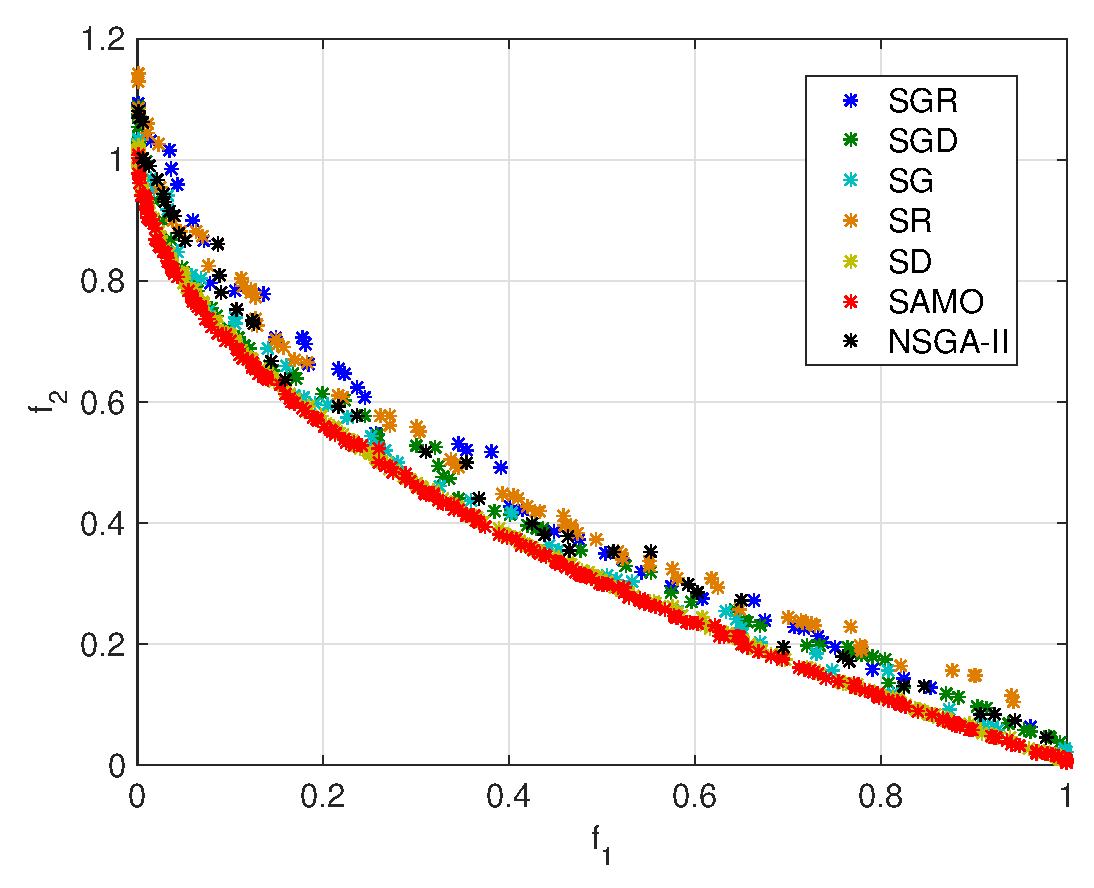
\includegraphics[width=.38\linewidth]{fig1a.eps}}\qquad
	\subfigure[Welded Beam]{\label{fig:welded_beam2_Pf}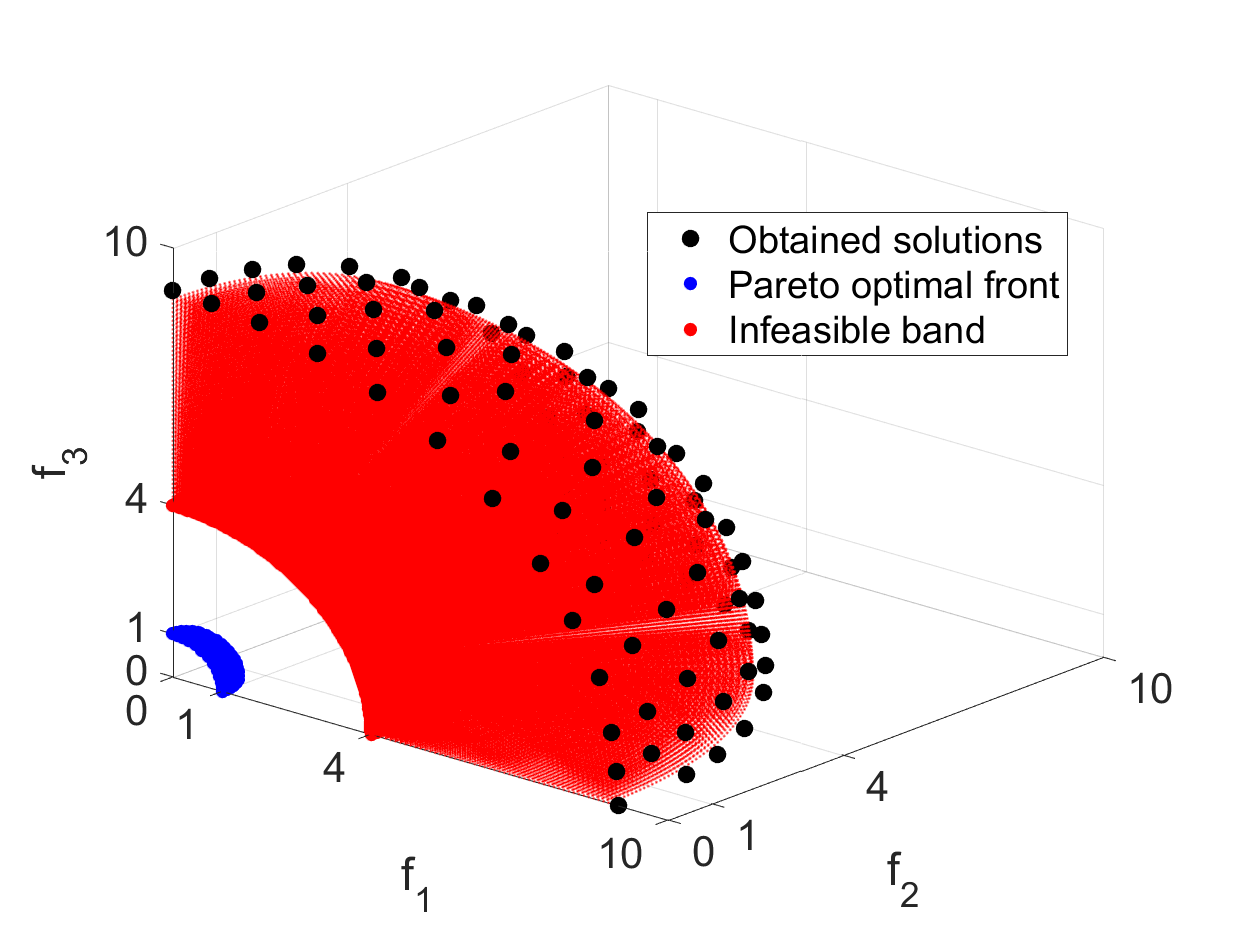
\includegraphics[width=.38\linewidth]{fig1b.eps}}\\
	\subfigure[CNC Machining]{\label{fig:metal_cutting2_Pf}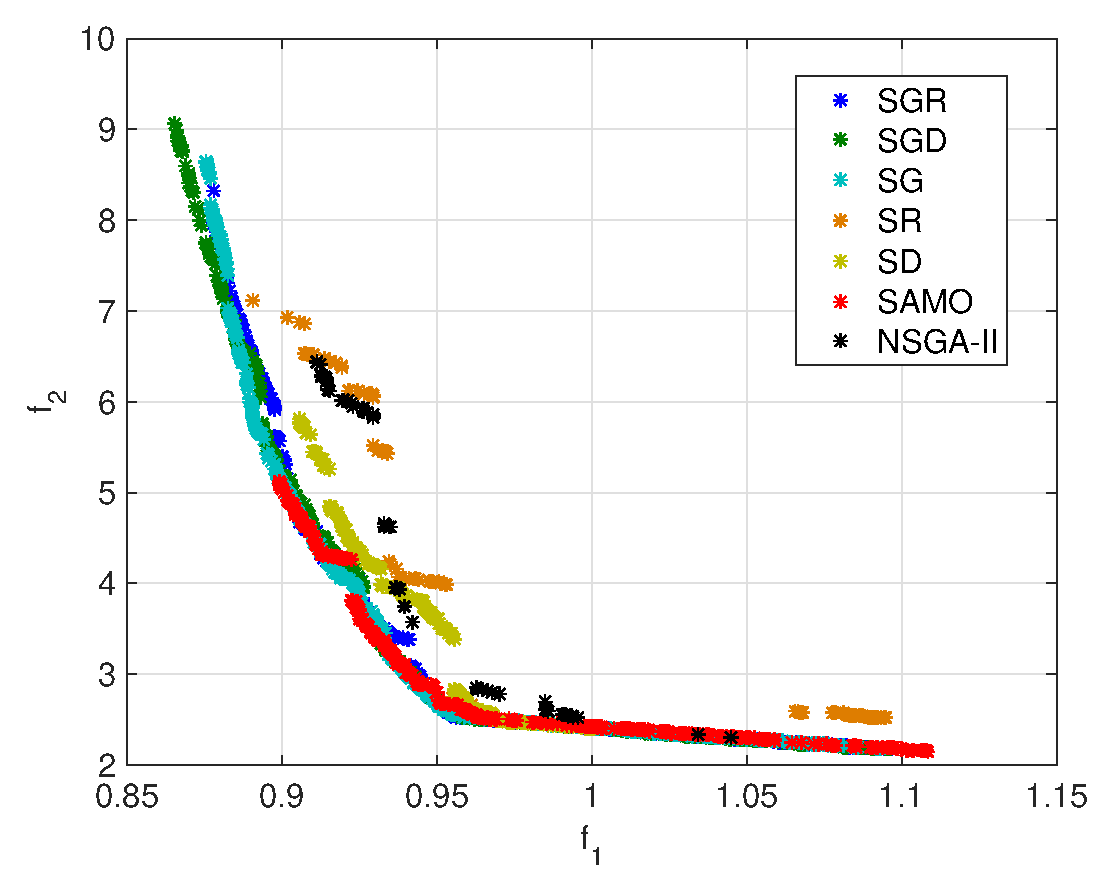
\includegraphics[width=.38\linewidth]{fig1c.eps}}\qquad
	\subfigure[Tool Spindle Design]{\label{fig:tool_spindle_Pf}\includegraphics[width=.38\linewidth]{fig1d.eps}}\\
	\subfigure[Metal Cutting]{\label{fig:metal_cutting3_Pf}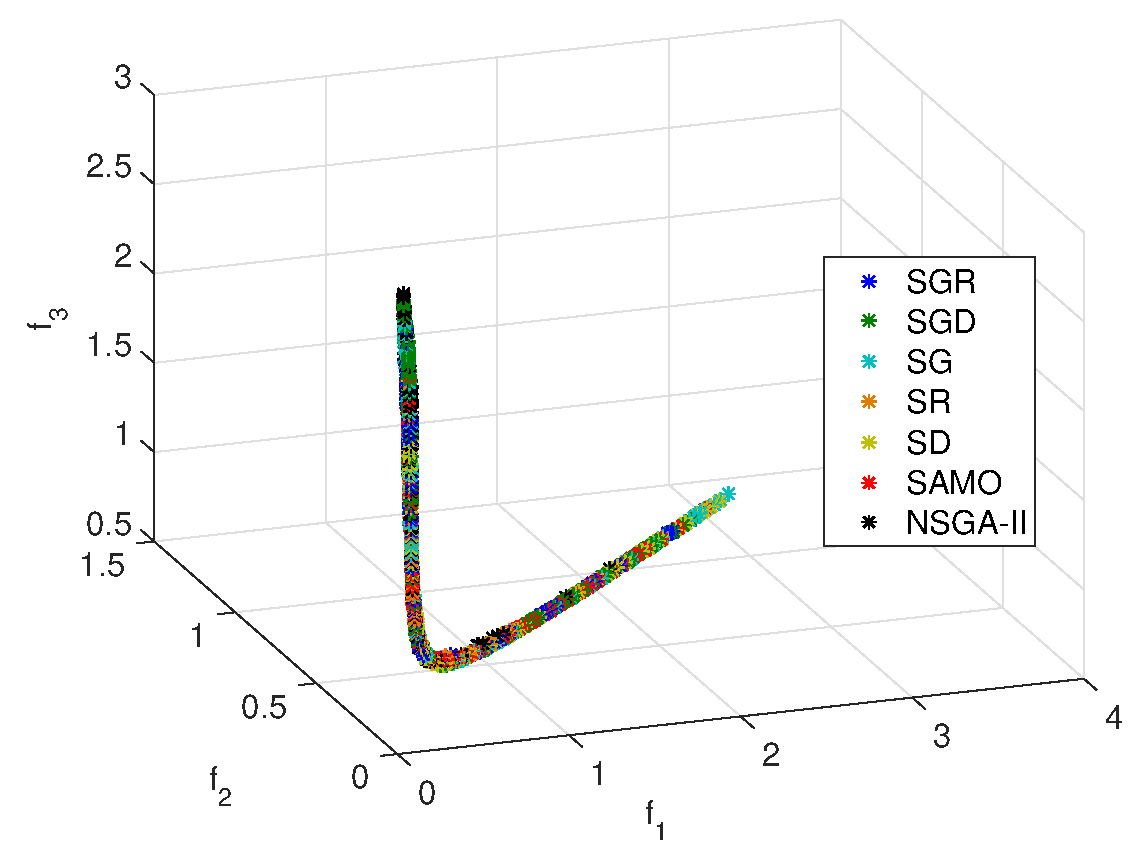
\includegraphics[width=.38\linewidth]{fig1e.eps}}\qquad
	\subfigure[PHEV Design]{\label{fig:PHEV_design_Pf}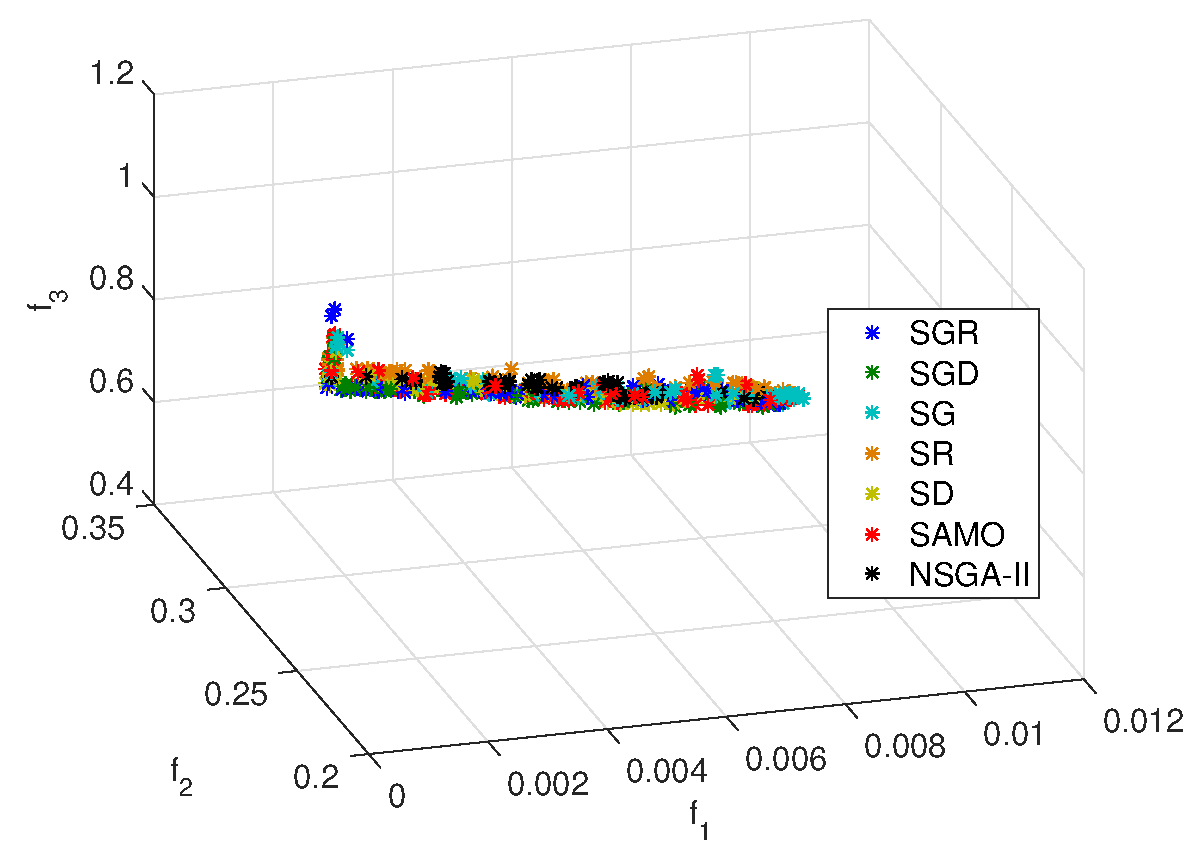
\includegraphics[width=.38\linewidth]{fig1f.eps}}\\
	\subfigure[Crash Safety Design]{\label{fig:Car_Crash_Pf}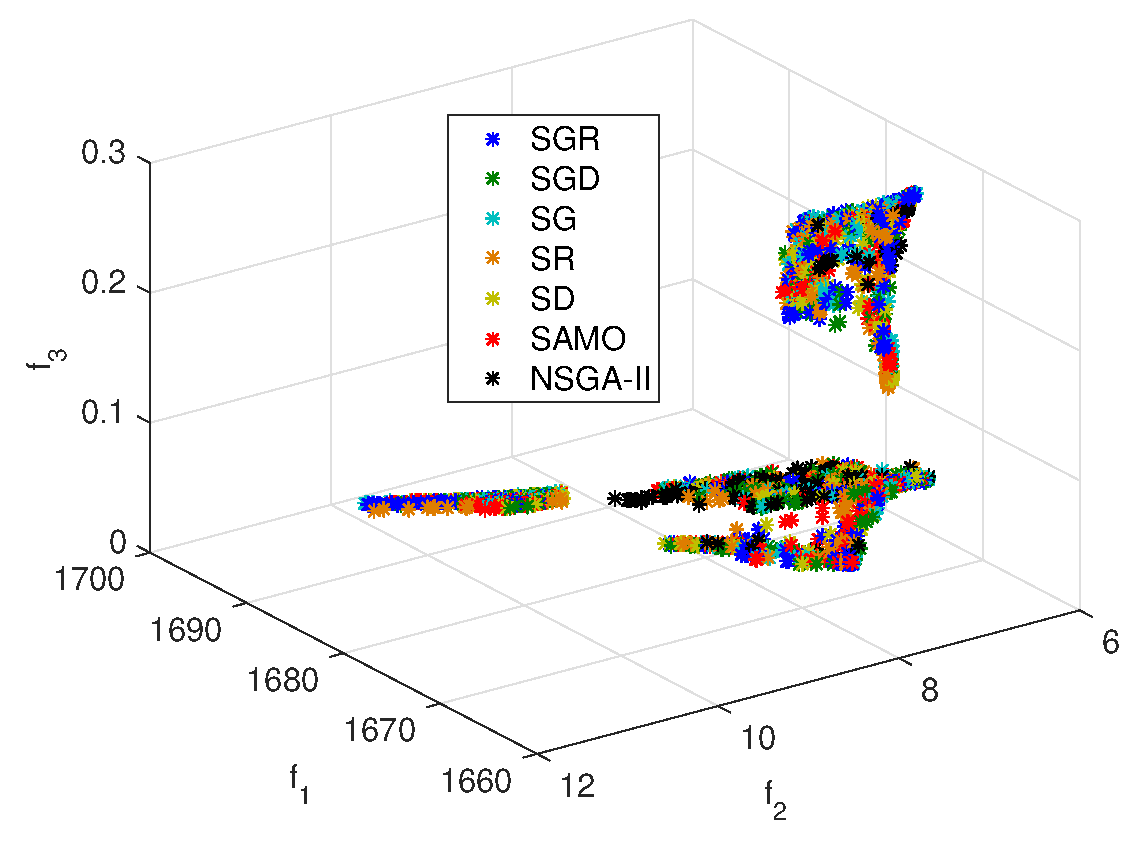
\includegraphics[width=.38\linewidth]{fig1g.eps}}\qquad
	\subfigure[Bulk Carrier Design]{\label{fig:bulk_carrier_design_Pf}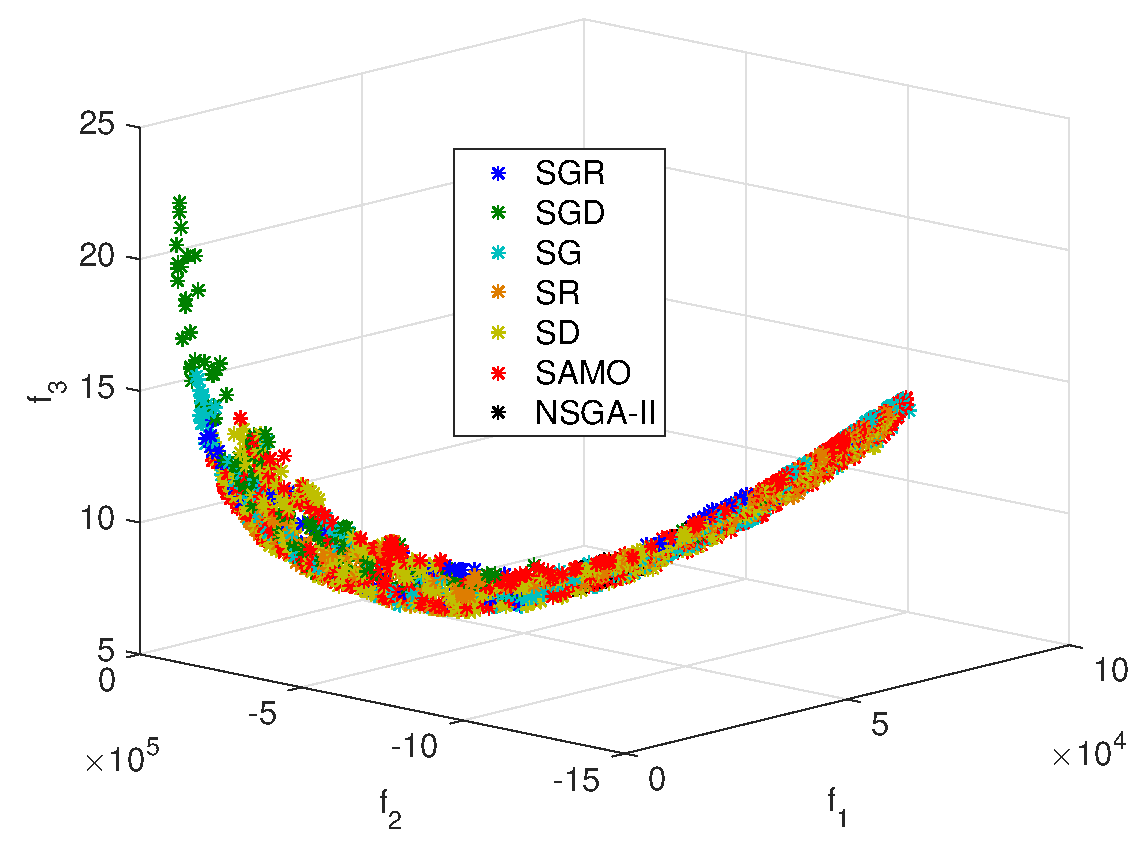
\includegraphics[width=.38\linewidth]{fig1h.eps}}\\
	\caption{Non-dominated front for median HV run}
	\label{fig:all_Pareto}
\end{figure*}

\begin{figure*}[!htb]
	\centering
	\subfigure[ZDT1]{\label{fig:zdt1_HV}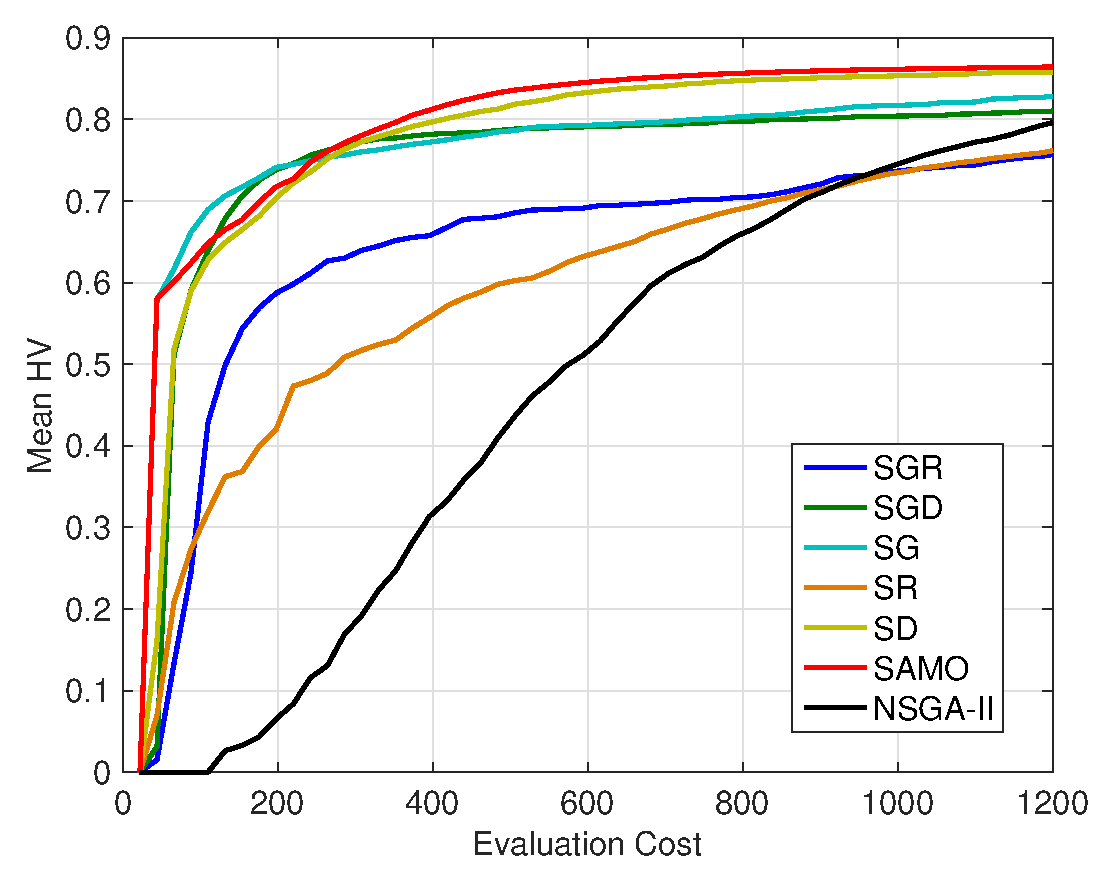
\includegraphics[width=.38\linewidth]{fig2a.eps}}\qquad
	\subfigure[Welded Beam]{\label{fig:welded_beam2_HV}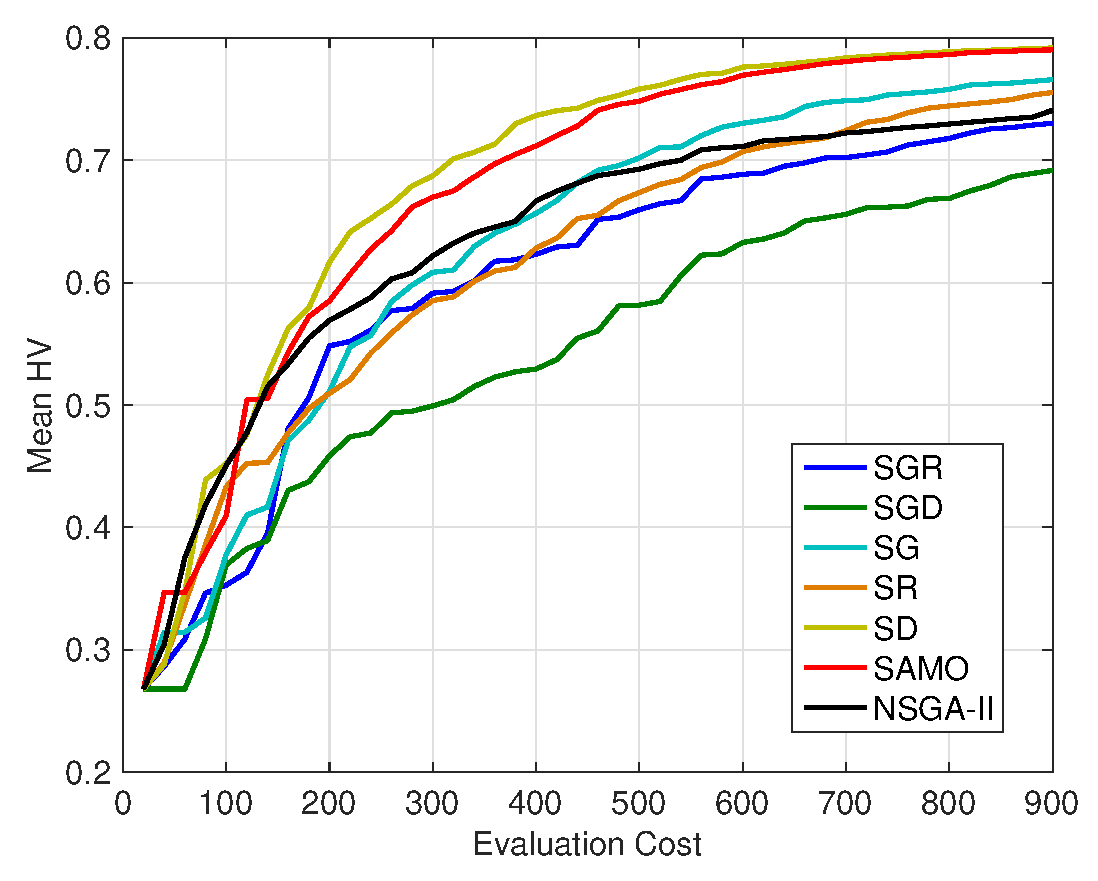
\includegraphics[width=.38\linewidth]{fig2b.eps}}\\
	\subfigure[CNC Machining]{\label{fig:metal_cutting2_HV}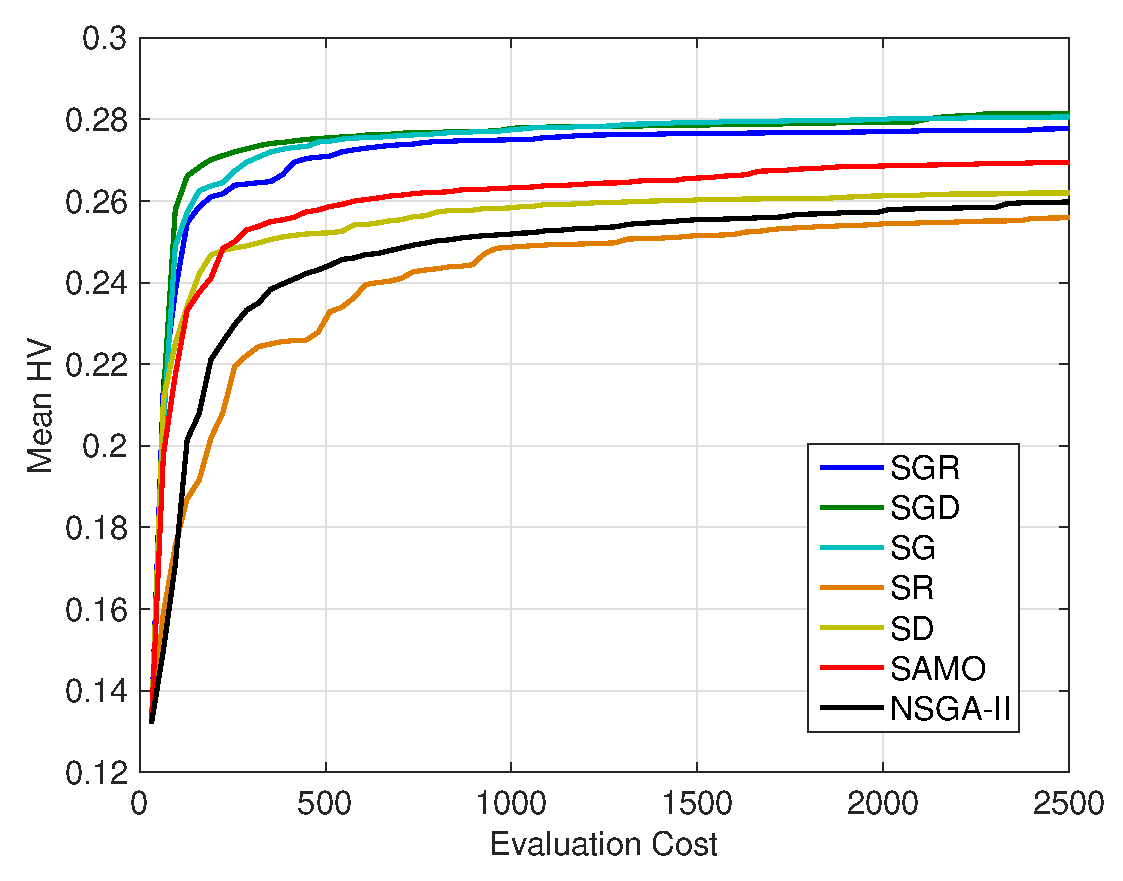
\includegraphics[width=.38\linewidth]{fig2c.eps}}\qquad
	\subfigure[Tool Spindle Design]{\label{fig:tool_spindle_HV}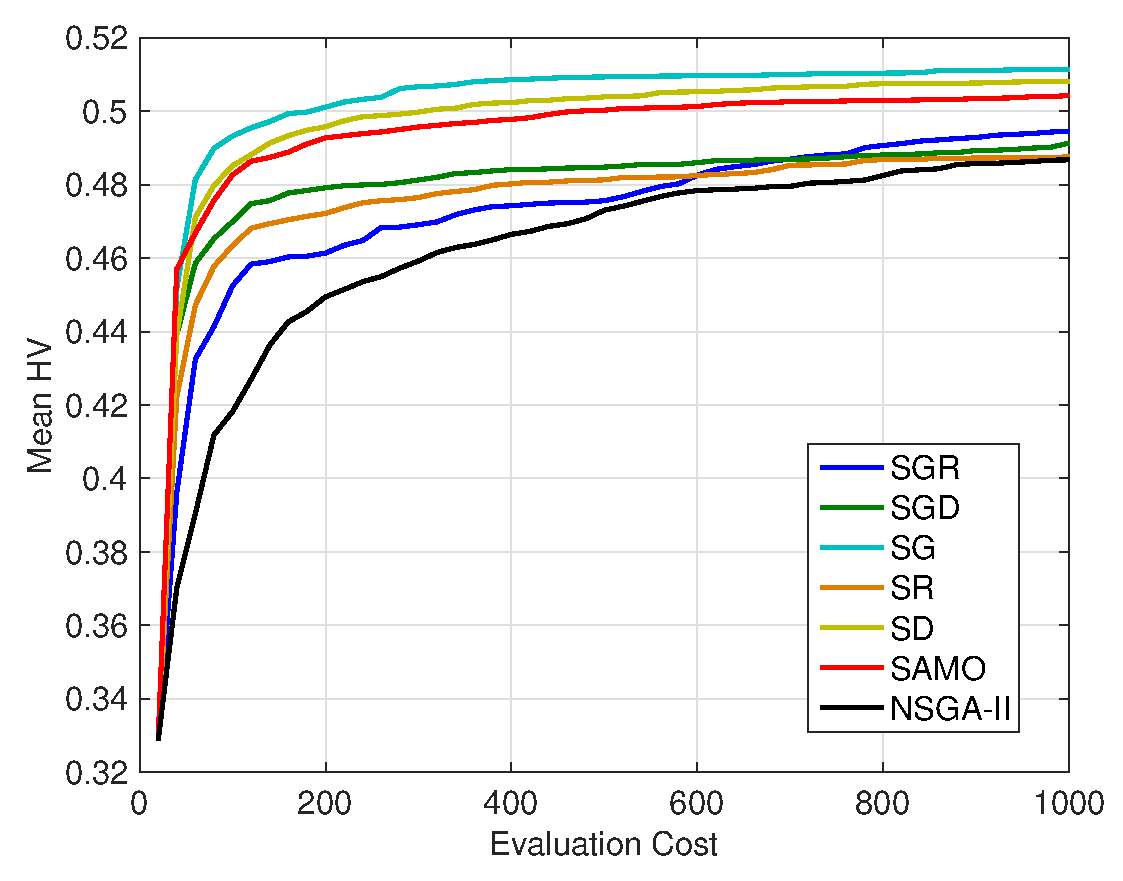
\includegraphics[width=.38\linewidth]{fig2d.eps}}\\
	\subfigure[Metal Cutting]{\label{fig:metal_cutting3_HV}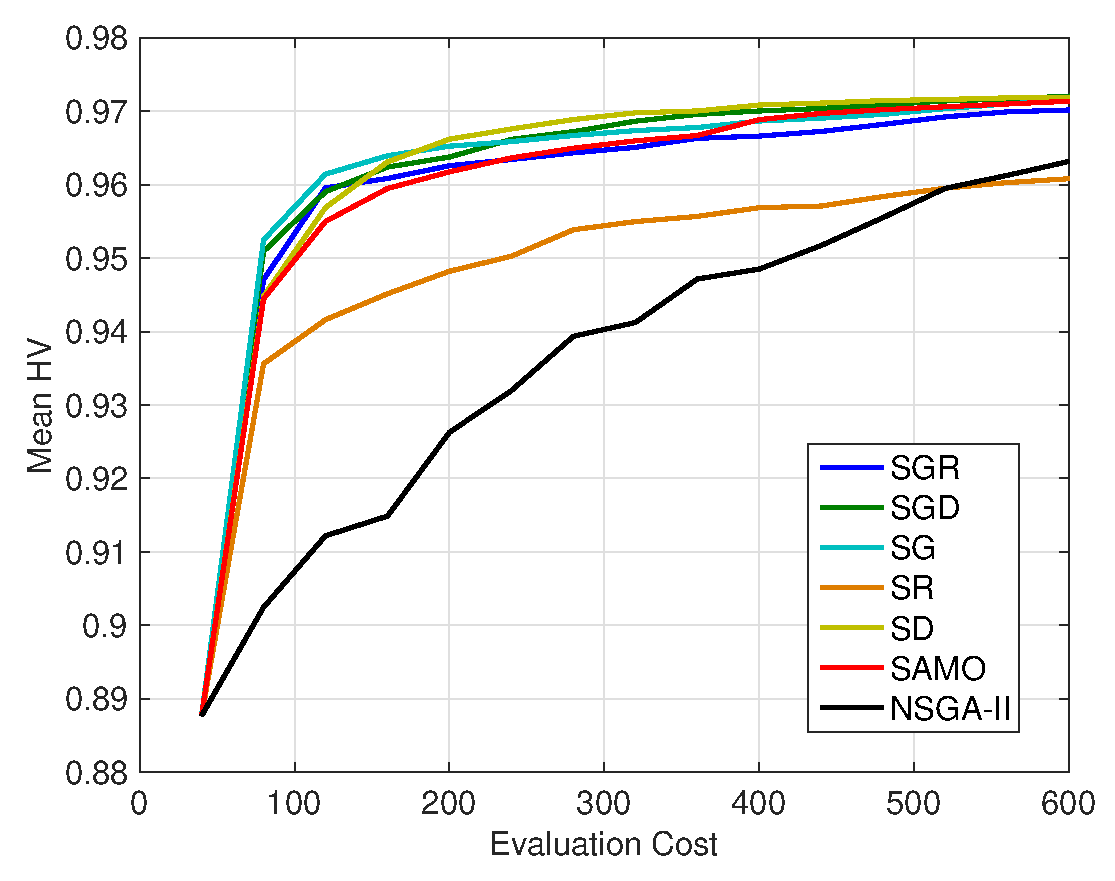
\includegraphics[width=.38\linewidth]{fig2e.eps}}\qquad
	\subfigure[PHEV Design]{\label{fig:PHEV_design_HV}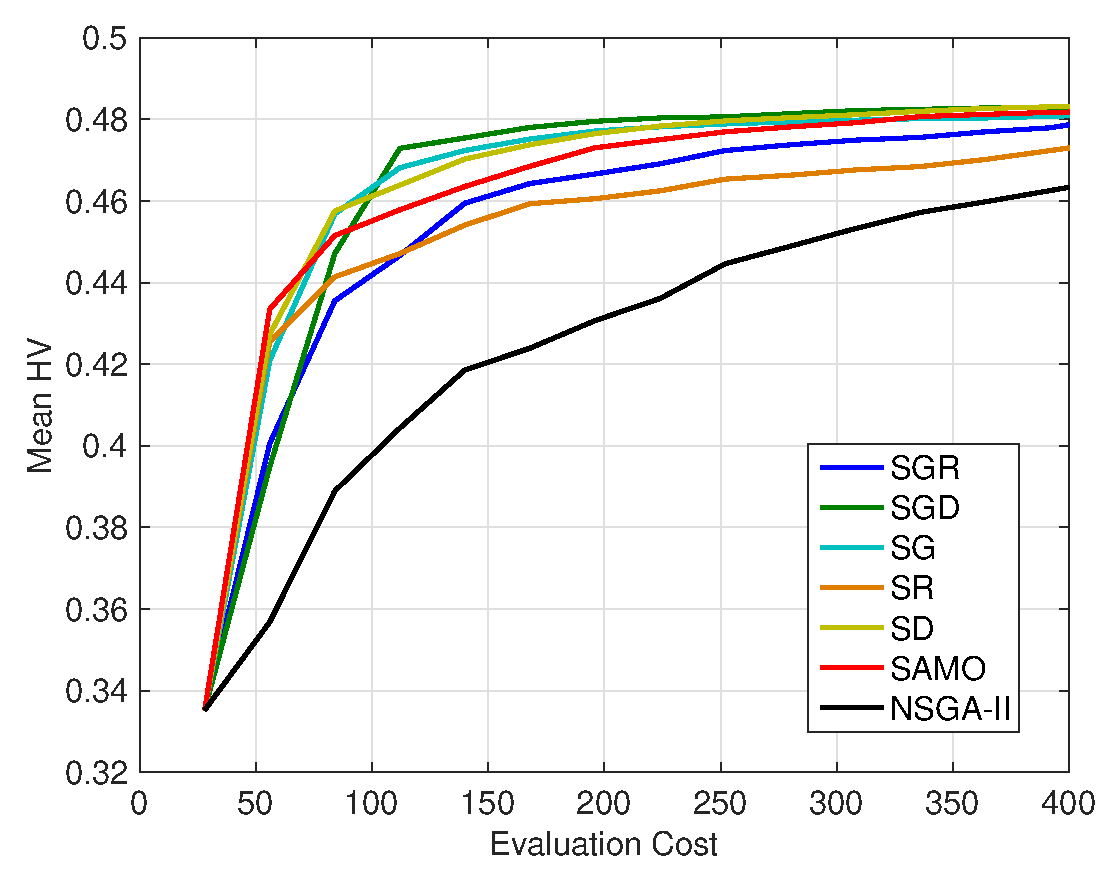
\includegraphics[width=.38\linewidth]{fig2f.eps}}\\
	\subfigure[Crash Safety Design]{\label{fig:Car_Crash_HV}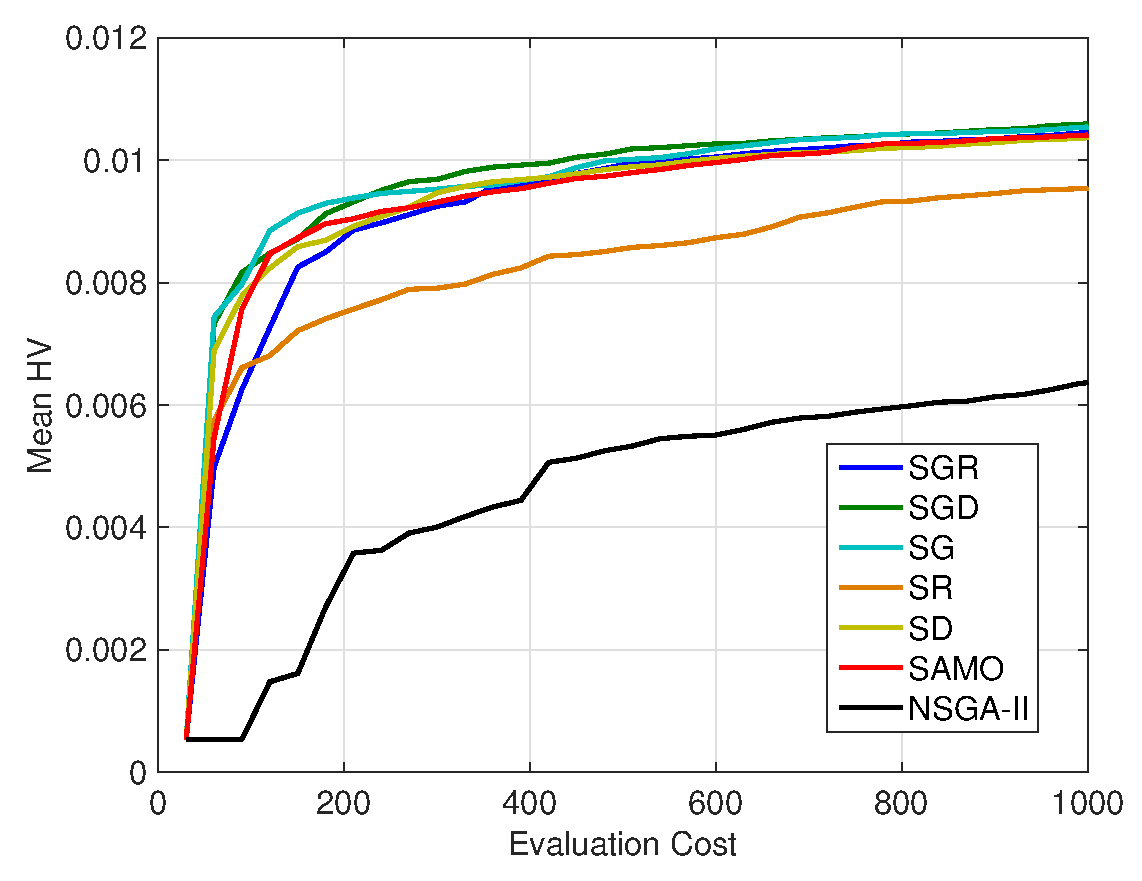
\includegraphics[width=.38\linewidth]{fig2g.eps}}\qquad
	\subfigure[Bulk Carrier Design]{\label{fig:bulk_carrier_design_HV}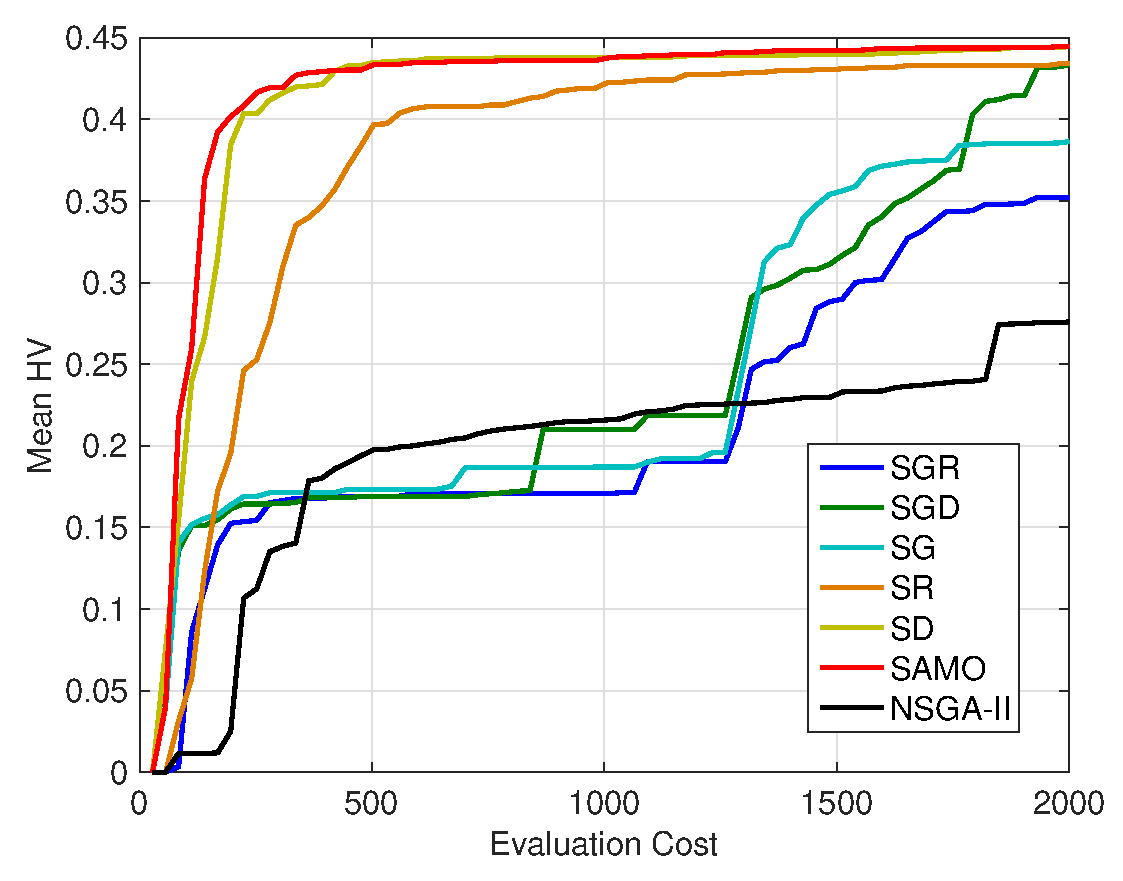
\includegraphics[width=.38\linewidth]{fig2h.eps}}\\
	\caption{Mean HV convergence}
	\label{fig:all_HV}
\end{figure*}
\clearpage
\subsection{Performance Comparison}

The reference points used for HV computation are listed in Table~\ref{tab:refprob1}. It is important to take note the mean HVs are plotted in the rate of convergence plots. The computation of HV and IGD statistics~(reported in Table~\ref{tab:hvigdstat1} for bi-objective problems and Table~\ref{tab:hvigdstat2} for tri-objective problems and all the convergence plots presented earlier) is based on all actual solutions evaluated until the given point in the search by SAMO, other variants and NSGA-II. Best HV and IGD statistics based on median statistics are marked in bold.

\begin{table*}[!htb]\scriptsize
	\centering
	\caption{Reference points for Hypervolume computation}
	\begin{tabular}{|l|l|l|l|l|}
		\noalign{\smallskip}\hline
		\textbf{Problems~(bi-objective)}         & \textbf{ZDT1} & \textbf{Welded Beam} & \textbf{CNC Machining} & \textbf{Tool Spindle Design}\\ \hline
		\textbf{Reference Points} & {[}1,1{]}   & {[}40,0.016{]}   & {[}1.15,10{]}  & {[}1.8E06,0.04{]} \\ \hline
		\textbf{Problems~(tri-objective)}         & \textbf{Metal Cutting} & \textbf{PHEV Design}  & \textbf{Car Crash} & \textbf{Bulk Carrier Design}\\ \hline
		\textbf{Reference Points} & {[}4,2,3{]} & {[}0.05,0.5,1.5{]} & {[}1699,6.9,0.3{]} & {[}6E04,-8E05,13{]}\\ \hline
	\end{tabular}
	\label{tab:refprob1}
\end{table*}

\begin{table*}[!htb]\scriptsize
	\centering
	\caption{HV and IGD statistics for bi-objective problems based on 10 independent optimization runs}
	\begin{tabular}{|l|l|l|l|l|l|l|l|l|l|l|l|}
		\noalign{\smallskip}\hline
		\multicolumn{2}{|c|}{} & \multicolumn{5}{|c|}{\textbf{Hypervolume}} & \multicolumn{5}{|c|}{\textbf{Inverted Generational Distance}}\\ \hline
		\textbf{Problems}            & \textbf{Algorithms} & \textbf{Best} & \textbf{Mean} & \textbf{Median} & \textbf{Worst} & \textbf{Std.} & \textbf{Best} & \textbf{Mean} & \textbf{Median} & \textbf{Worst} & \textbf{Std.}\\ \hline
		\multirow{7}{*}{\textbf{ZDT1}}                    & SGR                 & 0.8296         & 0.7571         & 0.7794           & 0.5525          & 0.0258              & 0.0208         & 0.0690         & 0.0478           & 0.2066          & 0.0186              \\ 
		& SGD                 & 0.8419         & 0.8102         & 0.8152           & 0.7453          & 0.0087   & 0.0148         & 0.0382         & 0.0298           & 0.1081          & 0.0088                    \\ 
		& SG                  & 0.8433         & 0.8285         & 0.8295           & 0.8139          & 0.0031     & 0.0154         & 0.0222         & 0.0217           & 0.0301          & 0.0015                       \\ 
		& SR                  & 0.8238         & 0.7617         & 0.7726           & 0.6308          & 0.0190    & 0.0254         & 0.0692         & 0.0582           & 0.1967          & 0.0160                    \\ 
		& SD                  & 0.8631         & 0.8581         & 0.8603           & 0.8387          & 0.0023       & 0.0042         & 0.0073         & 0.0054           & 0.0241          & 0.0019                   \\ 
		& SAMO                & 0.8660         & 0.8642         & \textbf{0.8647}           & 0.8607          & 0.0005& 0.0028         & 0.0036         & \textbf{0.0035}           & 0.0052          & 0.0002              \\ 
		& NSGA-II             & 0.8394         & 0.7961         & 0.7986           & 0.7047          & 0.0115     & 0.0164         & 0.0406         & 0.0396           & 0.0874          & 0.0061                    \\ \hline
		\multirow{7}{*}{\textbf{Welded Beam}}                    & SGR                 & 0.7848         & 0.7302         & 0.7331           & 0.6777          & 0.0106 & 0.0139         & 0.0507         & 0.0504           & 0.0853          & 0.0066  \\          
		& SGD                 & 0.8006         & 0.6917         & 0.7631           & 0.3582          & 0.0499            & 0.0048         & 0.0788         & 0.0328           & 0.3132          & 0.0339             \\ 
		& SG                  & 0.7970         & 0.7657         & 0.7650           & 0.7304          & 0.0084           & 0.0071         & 0.0285         & 0.0314           & 0.0569          & 0.0058          \\ 
		& SR                  & 0.7812         & 0.7553         & 0.7561           & 0.7272          & 0.0058           & 0.0166         & 0.0382         & 0.0421           & 0.0544          & 0.0041             \\ 
		& SD                  & 0.7981         & 0.7917         & \textbf{0.7938}           & 0.7804          & 0.0017& 0.0066         & 0.0111         & \textbf{0.0092}           & 0.0183          & 0.0014               \\ 
		& SAMO                & 0.7973         & 0.7901         & 0.7913           & 0.7836          & 0.0015   & 0.0078         & 0.0116         & 0.0109           & 0.0169          & 0.0009             \\ 
		& NSGA-II             & 0.7863         & 0.7408         & 0.7659           & 0.6485          & 0.0167      & 0.0144         & 0.0522         & 0.0346           & 0.1179          & 0.0127           \\ \hline
		
		\multirow{7}{*}{\textbf{CNC Machining}}                    & SGR                 & 0.2851         & 0.2778         & 0.2803           & 0.2497          & 0.0033    & 0.0014         & 0.0115         & 0.0053           & 0.0439          & 0.0043                \\ 
		& SGD                 & 0.2862         & 0.2815         & \textbf{0.2827}           & 0.2717          & 0.0013     & 0.0017         & 0.0038         & \textbf{0.0034}           & 0.0073          & 0.0005              \\ 
		& SG                  & 0.2849         & 0.2807         & 0.2807           & 0.2754          & 0.0009               & 0.0013         & 0.0086         & 0.0040           & 0.0265          & 0.0026               \\ 
		& SR                  & 0.2652         & 0.2559         & 0.2579           & 0.2385          & 0.0028               & 0.0213         & 0.0404         & 0.0342           & 0.0828          & 0.0060             \\ 
		& SD                  & 0.2818         & 0.2620         & 0.2636           & 0.2338          & 0.0053           & 0.0041         & 0.0335         & 0.0366           & 0.0628          & 0.0066              \\ 
		& SAMO                & 0.2790         & 0.2694         & 0.2719           & 0.2536          & 0.0029         & 0.0081         & 0.0216         & 0.0187           & 0.0467          & 0.0042              \\
		& NSGA-II             & 0.2762         & 0.2598         & 0.2567           & 0.2402          & 0.0045        & 0.0199         & 0.0407         & 0.0354           & 0.0729          & 0.0054                \\ \hline
		
		\multirow{7}{*}{\textbf{Tool Spindle Design}}                   & SGR                 & 0.5096     & 0.4945     & 0.5003       & 0.4554      & 0.0051         & 0.0112     & 0.0442     & 0.0324       & 0.1044      & 0.0104            \\
		& SGD                 & 0.5069     & 0.4913     & 0.4921       & 0.4737      & 0.0034        & 0.0166     & 0.0359     & 0.0381       & 0.0507      & 0.0033          \\ 
		& SG                  & 0.5145     & 0.5114     & \textbf{0.5115}       & 0.5058      & 0.0009        & 0.0016     & 0.0051     & \textbf{0.0039}       & 0.0109      & 0.0011           \\ 
		& SR                  & 0.5026     & 0.4875     & 0.4914       & 0.4579      & 0.0047          & 0.0237     & 0.0498     & 0.0466       & 0.1002      & 0.0076         \\ 
		& SD                  & 0.5124     & 0.5081     & 0.5095       & 0.5012      & 0.0012        & 0.0036     & 0.0081     & 0.0062       & 0.0148      & 0.0014           \\ 
		& SAMO                & 0.5111     & 0.5043     & 0.5082       & 0.4763      & 0.0032      & 0.0061     & 0.0154     & 0.0088       & 0.0611      & 0.0053         \\ 
		& NSGA-II             & 0.5036     & 0.4868     & 0.4943       & 0.4217      & 0.0081        & 0.0126     & 0.0347     & 0.0234       & 0.0950      & 0.0086            \\ \hline
	\end{tabular}
	\label{tab:hvigdstat1}
\end{table*}


\begin{table*}[!htb]\scriptsize
	\centering
	\caption{HV and IGD statistics for tri-objective problems based on 10 independent optimization runs}
	\begin{tabular}{|l|l|l|l|l|l|l|l|l|l|l|l|}
		\noalign{\smallskip}\hline
		\multicolumn{2}{|c|}{} & \multicolumn{5}{|c|}{\textbf{Hypervolume}} & \multicolumn{5}{|c|}{\textbf{Inverted Generational Distance}}\\ \hline
		\textbf{Problems}            & \textbf{Algorithms} & \textbf{Best} & \textbf{Mean} & \textbf{Median} & \textbf{Worst} & \textbf{Std Error} & \textbf{Best} & \textbf{Mean} & \textbf{Median} & \textbf{Worst} & \textbf{Std Error}\\ \hline
		\multirow{7}{*}{\textbf{Metal Cutting}}                             & SGR                 & 0.9718        & 0.9702        & 0.9702          & 0.9685         & 0.0004       & 0.0040        & 0.0058        & 0.0054          & 0.0085         & 0.0005                   \\ 
		& SGD                 & 0.9728        & 0.9721        & \textbf{0.9721}          & 0.9709         & 0.0002           & 0.0035        & 0.0048        & 0.0044          & 0.0098         & 0.0006                    \\ 
		& SG                  & 0.9725        & 0.9715        & 0.9716          & 0.9703         & 0.0002              & 0.0031        & 0.0037        & \textbf{0.0036}          & 0.0048         & 0.0002            \\ 
		& SR                  & 0.9702        & 0.9608        & 0.9624          & 0.9426         & 0.0026        & 0.0110        & 0.0234        & 0.0268          & 0.0336         & 0.0028               \\ 
		& SD                  & 0.9726        & 0.9719        & 0.9719          & 0.9704         & 0.0002         & 0.0054        & 0.0095        & 0.0092          & 0.0147         & 0.0011               \\ 
		& SAMO                & 0.9726        & 0.9714        & 0.9714          & 0.9705         & 0.0002        & 0.0047        & 0.0089        & 0.0090          & 0.0131         & 0.0008               \\ 
		& NSGA-II             & 0.9712        & 0.9632        & 0.9631          & 0.9557         & 0.0016            & 0.0065        & 0.0170        & 0.0148          & 0.0299         & 0.0030               \\ \hline
		\multirow{7}{*}{\textbf{PHEV Design}}                            & SGR                 & 0.4823         & 0.4787         & 0.4807           & 0.4701          & 0.0013        & 0.0059         & 0.0093         & 0.0082           & 0.0151          & 0.0009                   \\ 
		& SGD                 & 0.4848         & 0.4831         & \textbf{0.4837}           & 0.4799          & 0.0005        & 0.0046         & 0.0060         & \textbf{0.0053}           & 0.0096          & 0.0006              \\ 
		& SG                  & 0.4846         & 0.4809         & 0.4819           & 0.4767          & 0.0010        & 0.0039         & 0.0075         & 0.0070           & 0.0122          & 0.0008               \\ 
		& SR                  & 0.4788         & 0.4730         & 0.4744           & 0.4635          & 0.0017  & 0.0077         & 0.0145         & 0.0146           & 0.0239          & 0.0015               \\ 
		& SD                  & 0.4858         & 0.4832         & 0.4830           & 0.4808          & 0.0005 & 0.0031         & 0.0060         & 0.0057           & 0.0102          & 0.0006               \\ 
		& SAMO                & 0.4844         & 0.4818         & 0.4816           & 0.4788          & 0.0005         & 0.0048         & 0.0069         & 0.0064           & 0.0102          & 0.0005               \\ 
		& NSGA-II             & 0.4757         & 0.4634         & 0.4662           & 0.4379          & 0.0036    & 0.0110         & 0.0231         & 0.0197           & 0.0502          & 0.0034               \\ \hline						
		\multirow{7}{*}{\textbf{Car Crash}}                             & SGR                 & 0.0107         & 0.0105         & 0.0105           & 0.0101          & 0.0005           & 0.0032         & 0.0052         & 0.0053           & 0.0063          & 0.0003                 \\ 
		& SGD                 & 0.0107         & 0.0106         & \textbf{0.0106}           & 0.0105          & 0.0003            & 0.0043         & 0.0052         & 0.0052           & 0.0058          & 0.0001              \\ 
		& SG                  & 0.0107         & 0.0105         & \textbf{0.0106}           & 0.0103          & 0.0004            & 0.0040         & 0.0050         & \textbf{0.0048}           & 0.0064          & 0.0002               \\ 
		& SR                  & 0.0104         & 0.0095         & 0.0098           & 0.0076          & 0.0003           & 0.0057         & 0.0126         & 0.0090           & 0.0355          & 0.0030              \\ 
		& SD                  & 0.0107         & 0.0104         & 0.0103           & 0.0101          & 0.0006           & 0.0039         & 0.0060         & 0.0061           & 0.0084          & 0.0004              \\ 
		& SAMO                & 0.0108         & 0.0104         & 0.0103           & 0.0101          & 0.0008         & 0.0035         & 0.0058         & 0.0059           & 0.0072          & 0.0003               \\ 
		& NSGA-II             & 0.0106         & 0.0064         & 0.0087           & 0.0000          & 0.0014        & 0.0076         & 0.0289         & 0.0161           & 0.1019          & 0.0105              \\ \hline
		\multirow{7}{*}{\textbf{Bulk Carrier Design}}                             & SGR                 & 0.4544     & 0.3523     & 0.4338       & 0.0000      & 0.0564      & 0.0094     & 0.0577     & 0.0130       & 0.3971      & 0.0403        \\ 
		& SGD                 & 0.4478     & 0.4338     & 0.4384       & 0.4093      & 0.0042           & 0.0086     & 0.0218     & 0.0133       & 0.0578      & 0.0059           \\ 
		& SG                  & 0.4528     & 0.3869     & 0.4327       & 0.0000      & 0.0434           & 0.0081     & 0.0127     & 0.0120       & 0.0195      & 0.0012          \\ 
		& SR                  & 0.4455     & 0.4344     & 0.4322       & 0.4227      & 0.0022             & 0.0105     & 0.0122     & 0.0121       & 0.0142      & 0.0004           \\ 
		& SD                  & 0.4512     & 0.4445     & 0.4452       & 0.4311      & 0.0019       & 0.0080     & 0.0097     & 0.0099       & 0.0111      & 0.0003        \\ 
		& SAMO                & 0.4499     & 0.4447     & \textbf{0.4454}       & 0.4381      & 0.0013      & 0.0085     & 0.0097     & \textbf{0.0097}       & 0.0110      & 0.0002         \\ 
		& NSGA-II             & 0.4052     & 0.2759     & 0.3075       & 0.0729      & 0.0341       & 0.0713     & 0.1659     & 0.1232       & 0.3534      & 0.0279             \\ \hline
	\end{tabular}
	\label{tab:hvigdstat2}
\end{table*}


\begin{figure*}[ht]
	\centering
	\subfigure[]{\label{fig:HVperf}\includegraphics[width=.38\linewidth]{fig3a.eps}}\qquad
	\subfigure[]{\label{fig:IGDperf}\includegraphics[width=.38\linewidth]{fig3b.eps}}
	\caption{Performance profile: (a) Median (inverse of) HV statistics (b) Median IGD statistics}
	\label{fig:Perfprofile}
\end{figure*}

Performance profiles can be used to identify the most appropriate algorithm that is statistically preferred to solve problems belonging to the class. The observations based on median HV and IGD statistics are summarized using performance profile plots in Figure~\ref{fig:Perfprofile}, where Figure~\ref{fig:HVperf} is based on median HV statistics and Figure \ref{fig:IGDperf} is based on median IGD statistics achieved using different algorithms across all problems.

From the performance profile plot based on median HV statistics presented in Figure~\ref{fig:HVperf} the observations are listed below:

\begin{enumerate} 
	
	\item SAMO performs the best or close to the best ($\tau \approx$ 1) for 75\% of the problems). This observation can be confirmed from Table~\ref{tab:hvigdstat1} and Table~\ref{tab:hvigdstat2} where SAMO performs best in two out of eight problems. Among the remaining six problems, performance of SAMO is almost at par in four problems compared to the performance delivered by the best algorithm. For the remaining two problems, performances of SAMO are marginally worse than the best performances. Performances of SD and SG are very close to the best except in one problem for SD and two problems for SG where they are significantly worse. Similarly SGD delivers almost at par performances with the best one for about 50\% of the problems and it significantly deteriorates thereafter.
	\item Since $\rho_{SGR}(1)$ = 0, $\rho_{SR}(1)$ = 0 and $\rho_{NSGA-II}(1)$ = 0, SGR, SR and NSGA-II are never the best in terms of median HV statistics for this set of problems. SGR performs better than SG and SGD in one problem and worse than SAMO and SD in all the problems. Performances delivered by SR and NSGA-II are worse than all the other variants for all the problems, with SR in general showing better performance among these two. 
	\item One can calculate from Figure~\ref{fig:HVperf} that area under the curves (AUC), $AUC_{SAMO}$ = 0.4406, $AUC_{SD}$ = 0.4390, $AUC_{SR}$ = 0.3984, $AUC_{SG}$ = 0.4353, $AUC_{SGD}$ = 0.4326, $AUC_{SGR}$ = 0.4214 and $AUC_{NSGA-II}$ = 0.3541. Since, $AUC_{SAMO} > AUC_{SD} > AUC_{SG} > AUC_{SGD} > AUC_{SGR} > AUC_{SR} > AUC_{NSGA-II}$ algorithm SAMO is the most efficient one followed by SD and others. One can also notice that use of local surrogates in general delivers better results compared to those obtained using global surrogates except in the context of dealing with radial basis function. Notably, within local surrogates SAMO is most reliable and efficient and within global surrogates SG is the most reliable and efficient one. This fact can be accounted for dealing with multiple types of surrogates instead of a single one. However, NSGA-II performs worst among all since it is run without any surrogates. 
\end{enumerate}

Similarly from Figure~\ref{fig:IGDperf} based on median IGD statistics the observations are summarized below:

\begin{enumerate} 
	
	\item SAMO performs best or at par~($\tau\approx$ 1) for 62.5\%~(5 out of 8) of the problems. In 25\% of the problems, SAMO performs best which can be confirmed from  Table~\ref{tab:hvigdstat1} and Table~\ref{tab:hvigdstat2}. For three problems, SAMO performs relatively worse compared to the performances delivered by best algorithm, but the factor $\tau$ remains relatively low compared to most other variants. Performance of SG is better than that of SD for six out of eight problems. In one problem SD delivers significantly worse performance compared to SG and SAMO. Similarly SGD delivers almost at par performances with the best one for about 62.5\% of the problems and it significantly deteriorates thereafter.
	\item Since $\rho_{SGR}(1)$ = 0, $\rho_{SR}(1)$ = 0 and $\rho_{NSGA-II}(1)$ = 0, SGR, SR and NSGA-II are never the best in terms of median IGD statistics for this set of problems.  SGR performs better than SGD in one problem, and worse than SAMO, SD and SG in all the problems. Performances of SR are better or at par to those of NSGA-II in seven problems and significantly worse in one problem.
	\item One can calculate from Figure~\ref{fig:IGDperf} that $AUC_{SAMO}$ = 14.9790, $AUC_{SD}$ = 14.6847, $AUC_{SR}$ = 10.5820, $AUC_{SG}$ = 14.9552, $AUC_{SGD}$ = 13.7850, $AUC_{SGR}$ = 13.1484 and $AUC_{NSGA-II}$ = 10.3339. Since, $AUC_{SAMO} > AUC_{SG} > AUC_{SD} > AUC_{SGD} > AUC_{SGR} > AUC_{SR} > AUC_{NSGA-II}$ algorithm SAMO is the most efficient one followed by SG and others. Similar observations as based on HV statistics can be made except the fact that in terms of median IGD statistics SG performs better than SD.
\end{enumerate}

From the observations listed above for this set of problems, it can be concluded that SAMO is statistically the best choice among the set of local and global variants. The SAMO code is be made available for download from the authors' website \cite{MDOsamo}, so that it could be utilized by the research community for further studies and benchmarking.


\section{Conclusion and Future Work}
\label{sec:conc}

In this paper, a surrogate assisted optimization framework~(SAMO) has been presented for multi-objective optimization. The approach uses NSGA-II as the baseline algorithm and multiple local surrogates of different types to represent the objectives and constraints. The approach is easily extendable to other population based metaheuristics. The proposed SAMO performs actual evaluations in each generation, trains the local surrogate models of different types and runs NSGA-II within the bounds of the neighboring set for each offspring. The process attempts to identify a set of non-dominated solutions in different regions of the search space using the best surrogate~(one delivering the minimum MSE). This is in contrast to existing approaches which typically use only single surrogate in either local or global search space.

The approach offers the flexibility in the scenarios where a function~(objective or constraint) is better approximated using a particular surrogate in a region and a different surrogate in other regions of the search space. Furthermore, even in a neighborhood, the approach allows the constraints and objectives to be approximated using different surrogates. In order to maximize the use of information from all actual evaluations, the algorithm maintains an external archive that is used to train the surrogate models~(Kriging, Radial Basis Function, Multi-layer Perceptron, Response Surface Methodology of $1^{st}$ and $2^{nd}$ order). 

The performance of the proposed algorithm is compared with local and global surrogate forms to highlight the benefits. The performance profiles clearly suggest that SAMO is the best strategy for such classes of problems. The performance profiles also highlight the clear benefits of local surrogates. Among the global surrogates, use of the best global surrogate is better than opting for predefined surrogates. Although SAMO and other methods which maintain multiple surrogates incur additional computational cost for construction and re-training of surrogates, this cost is still insignificant~(compared to true evaluations) for problems where the evaluation of each candidate design requires expensive simulation(s), e.g. computational fluid dynamics, finite element analysis, etc. With greater flexibility offered through multiple surrogates, we expect the approach to become more attractive and beneficial for practical applications. 

\section{Summary and Future Directions}
\label{sec:sum}


\section{Conclusion}
\label{sec:conc}


\small
